\documentclass[aspectratio=43, 8pt,t]{beamer}
\graphicspath{{figures/}} % Setting the graphicspath

% Theme settings
\usetheme{Madrid}
\usecolortheme{default}
\setbeamertemplate{navigation symbols}{}   % removes navigation symbols such as 'next page'
\setbeamertemplate{footline}{}             % remove line with name, date, page nr.
\setbeamercolor*{frametitle}{bg=white}     % remove background from frametitle
\usepackage{caption}
% \captionsetup[figure]{labelformat=empty}% redefines the caption setup of the figures environment in the beamer class.
\setbeamersize{text margin left=20pt,text margin right=10pt}
\usefonttheme[onlymath]{serif} % makes beamer math look like article math
\usepackage{hyperref}
\usepackage{booktabs}

%======================= title page info =======================
\title{Intrinsic charm in the proton}
\date{Flavoured Jets at the LHC  \\[0.1cm] 12 June 2024, Durham}
\author{Roy Stegeman}
\institute{\small The University of Edinburgh}


%======================= page numbering =======================
\addtobeamertemplate{navigation symbols}{}{%
  \ifnum\thepage>1% don't display frame number on the first slide
    \usebeamerfont{footline}\insertframenumber\hspace*{2em}\vspace*{2em}% display frame number
  \fi%
}

%=================================== colors ====================================
\definecolor{RoyBlue}{RGB}{22, 46, 69}
\definecolor{RoyGrey}{RGB}{64, 88, 128}

\newcommand{\hlme}[1]{{\color{red}\bf #1}} % highlight me

\setbeamercolor{structure}{fg=RoyBlue} % itemize, enumerate, etc
\setbeamercolor{frametitle}{fg=RoyGrey}
\setbeamercolor{section in head/foot}{bg=RoyBlue}


%======================= add progress dots to headline =========================
% \setbeamertemplate{headline}{%
%     \begin{beamercolorbox}[ht=4mm,dp=4mm]{section in head/foot}
%         \insertnavigation{\paperwidth}
%     \end{beamercolorbox}%
% }%
% \makeatother


%======================= add section title page ================================
\newcommand{\SectionTitleFrame}[1][]{%
  \begin{frame}
    \vfill
    \centering
    \begin{beamercolorbox}[sep=8pt,center,shadow=true,rounded=true]{title}
      \usebeamerfont{title}\insertsection\par
    \end{beamercolorbox}
    % Include optional text if provided
    \ifx\relax#1\relax\else
      \vspace{0.5cm}
      \textbf{#1}
    \fi
    \vfill
  \end{frame}
}

% Use \SectionTitleFrame in \AtBeginSection
\AtBeginSection[]{
  \SectionTitleFrame
}


%=================================== titlepage =================================
\titlegraphic{\vspace*{6mm}
  
\includegraphics[height=1.5cm]{logos/edi_logo.png} \hspace{10mm}
  
\includegraphics[height=0.8cm]{logos/nnpdf_logo_official.pdf} \hspace{10mm}
  
\includegraphics[height=1.5cm]{logos/higgs_logo.jpg}
}

\defbeamertemplate{title page}{noinstitute}[1][]
{
  \vbox{}
  \vfill
  \begingroup
    \centering
    \begin{beamercolorbox}[sep=8pt,center,#1]{title}
      \usebeamerfont{title}\inserttitle\par%
      \ifx\insertsubtitle\@empty%
      \else%
        \vskip0.25em%
        {\usebeamerfont{subtitle}\usebeamercolor[fg]{subtitle}\insertsubtitle\par}%
      \fi%
    \end{beamercolorbox}%
    \vskip2em\par
    \begin{beamercolorbox}[sep=0pt,center,#1]{author}
      \usebeamerfont{author}\insertauthor
    \end{beamercolorbox}
  \begin{beamercolorbox}[sep=0pt,center,#1]{author}
    \usebeamerfont{institute}\insertinstitute
  \end{beamercolorbox}
  \vspace*{8pt}
  \vspace*{16pt}
    \begin{beamercolorbox}[sep=0pt,center,#1]{date}
      \usebeamerfont{date}\insertdate
    \end{beamercolorbox}\vskip0.5em
    {\usebeamercolor[fg]{titlegraphic}\inserttitlegraphic\par}
  \endgroup
  \vfill
}

\makeatletter
\setbeamertemplate{title page}[noinstitute][colsep=-4bp,rounded=true,shadow=\beamer@themerounded@shadow]
\makeatother


\begin{document}
{
\setbeamertemplate{headline}{} % remove headline from titlepage
\begin{frame}
  \titlepage
\end{frame}
}

\setbeamertemplate{enumerate items}[default]

\pgfdeclarelayer{bg}    % declare background layer
\pgfsetlayers{bg,main}  % set the order of the layers (main is the standard layer)


% SLIDES =======================================================================
\newcommand{\nn}{\vspace*{1em}}

% PLAN FOR THE TALK

% mostly IC talk
% nFONLL thanks to simultaneous PDF feature in EKO
% emphasize evidence increases at N3LO AND with MHOUs, while evidence for valence remains the same
% a couple of slides on the pheno study
% future developments and data?

% W+c-jet to probe strange PDF: https://arxiv.org/pdf/2009.00014
% contain [ATLAS (1402.6263)] and  [CMS (1310.1138)] 7 TeV data
% see Stagnitto GGI talk: https://www.ggi.infn.it/talkfiles/slides/slides6682.pdf

% D-meson asymmetries in Z+c-jet to probe IC valence PDF: https://arxiv.org/pdf/2311.00743
% The paper also suggests flavor-tagged structure functions at EIC, but that's not jets at LHC

% Z+c-jet for IC: https://arxiv.org/pdf/2208.08372


% Charm-tagged DIS at EIC in "measureing valence" slide
% comparison with models
% momentum fraction (TG)
% dataset dependence (TG)





\begin{frame}{Perturbative charm}
  A common assumption in PDF fits is that the proton wave function does not contain charm quarks but only light quarks

  \vspace*{1em}
  This assumption leads to a purely perturbative charm, namely:
  \begin{itemize}
    \item Charm quark pairs are perturbatively generated in DGLAP evolution\\
    $f_c^{(4)}\propto \alpha_s \log\left(\frac{Q^2}{m_c^2}\right)P_{qg} \otimes f_g^{(4)} + \mathcal{O}(\alpha_s^2)$

    \item Present only above the heavy quark threshold (in 4FNS)

    \item Fixed by the light flavour and gluon PDFs
  \end{itemize}

  \vspace*{1em}
  \only<2>{However instead of assuming charm completely perturbatively, one may determine it on the same footing as the light quarks}
\end{frame}


\begin{frame}{Fitted charm}
  NNPDF4.0 independently parametrizes the total charm distribution $c^+=c+\bar{c}$

  \vspace*{1em}
  Fitted charm is a combination of perturbative and intrinsic charm : \\
  $f_c^{(4)} = A_{ci}f_i^{(3)}+A_{cc}f_c^{}$
  \begin{itemize}
    \item in 4FNS charm is not fixed by light flavour PDFs
    \item Instead there is a contributing that is part of the static proton wave function
    \item Intrinsic component is present at all scales
  \end{itemize}

  \vspace*{1em}
  Intrinsic charm is charm in the 3FNS!

  \begin{figure}
    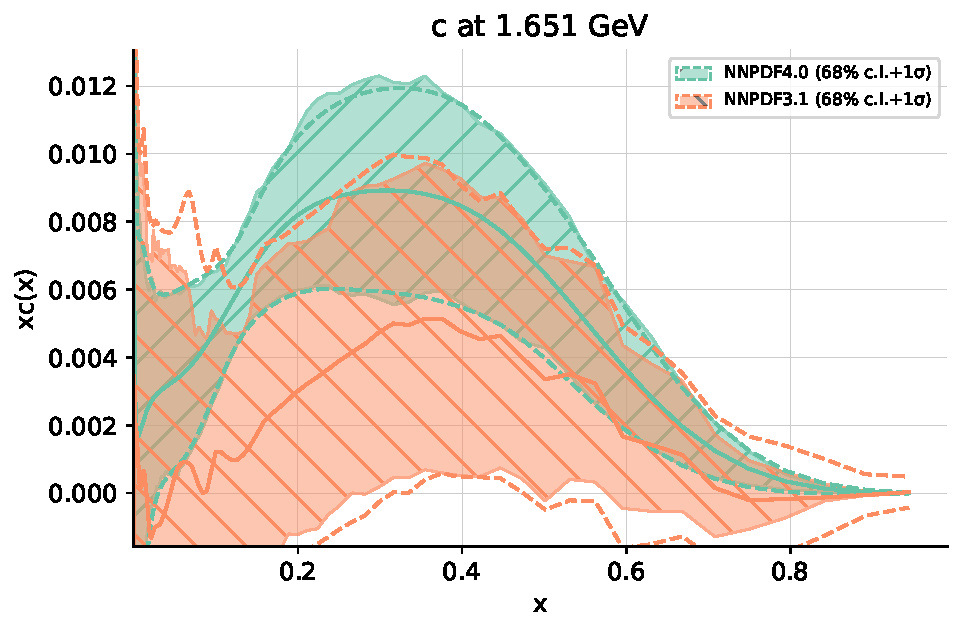
\includegraphics[width=0.5\textwidth]{nnpdf40_vs_nnpdf31.pdf}
    \caption*{4FNS}
  \end{figure}
\end{frame}

\begin{frame}{Fitted vs perturbative charm PDF}
  \begin{figure}
    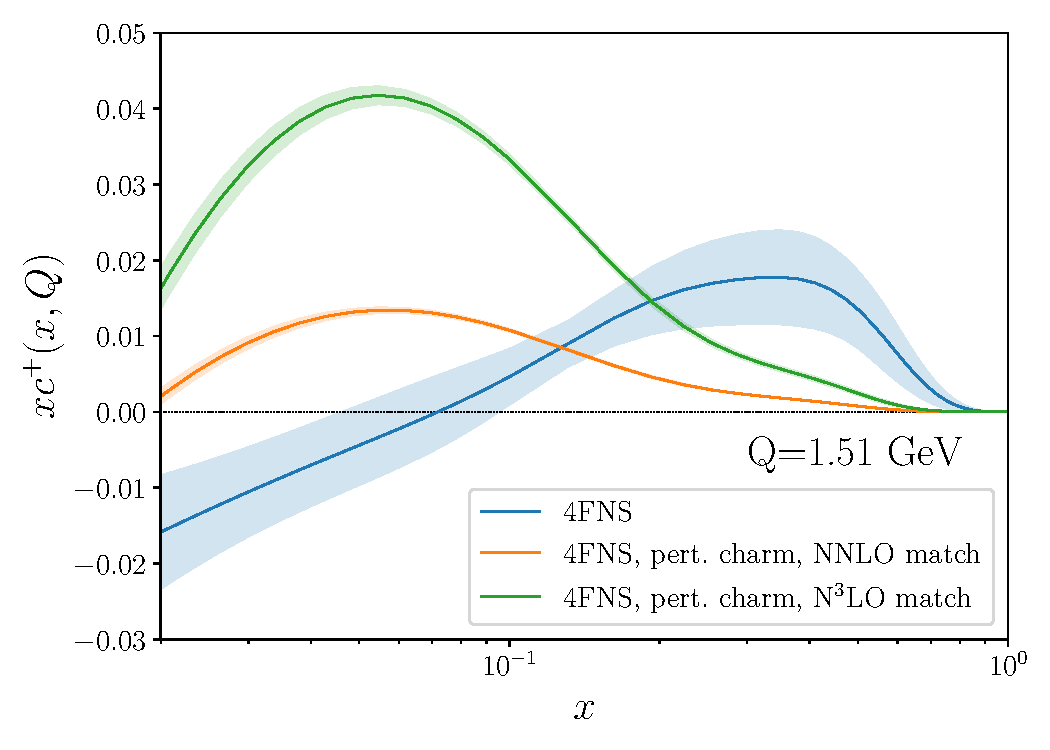
\includegraphics[width=0.6\textwidth]{pch_vs_fitted_forward.pdf}
  \end{figure}

  Fitted charm:
  \begin{itemize}
    \item independent of matching conditions
    \item stable upon variations of $m_c$
    \item Insensitive to MHOU
    \item Bump at large-$x$ where radiative charm production is limited
  \end{itemize}
\end{frame}


\begin{frame}{EKO and nFONLL}
  \begin{figure}
    
\includegraphics[width=0.6\textwidth]{eko_header.png}
  \end{figure}
  \begin{itemize}
    \item Impements DGLAP solutions up to aN3LO QCD and NLO QEC
    \item Supports coexising PDFs in different FNS at all scales
    \item[$\Rightarrow$] Construct FONLL with coexisting FNS PDFs
  \end{itemize}

  $$F_{FONLL} = F^{(4)}(m_c=0) + F^{(3)}(m_c) - \lim_{x\rightarrow 0} F^{(3)}(m_c)$$
\end{frame}


\section*{Evidence for intrinsic charm quarks in the proton}
\SectionTitleFrame[\hyperlink{https://arxiv.org/abs/2208.08372}{NNPDF, 2208.08372}]

\begin{frame}{How to determine intrinsic charm?}
  \begin{figure}
    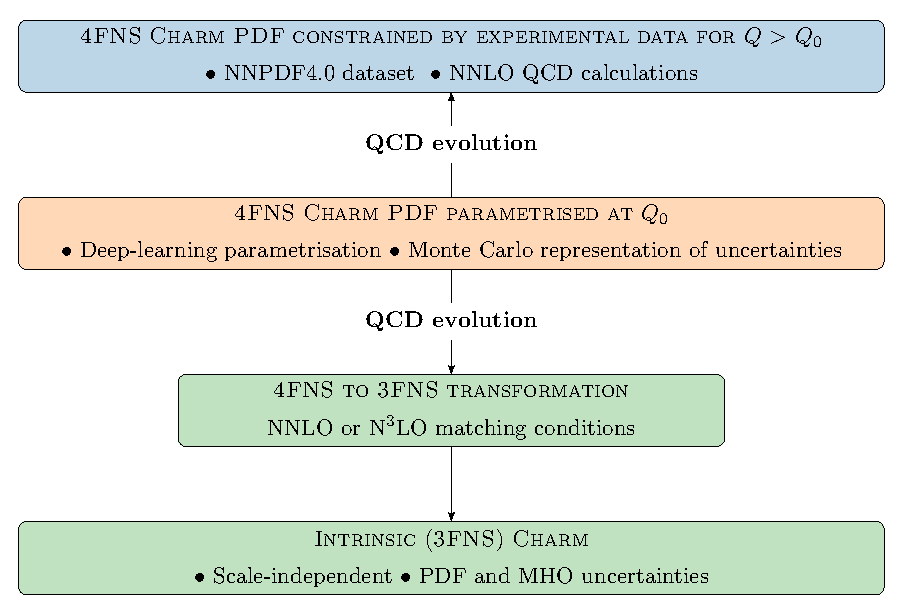
\includegraphics[width=0.6\textwidth]{strategy.pdf}
  \end{figure}

\end{frame}


\begin{frame}{Evidence for intrinsic charm (in 3FNS)}
  \begin{figure}
    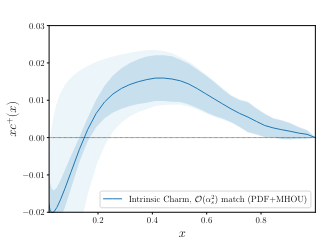
\includegraphics[width=0.5\textwidth]{discovery_of_ic.png}
  \end{figure}
  \begin{itemize}
    \item MHOU estimated from N3LO-NNLO matching difference
    \item Large perturbative uncertainty for small-$x$
    \item PDF dominated uncertainty at large-$x$
    \item Non-zero intrinsic charm peak
  \end{itemize}
\end{frame}

\begin{frame}{Z+charm at LHCb}
  \begin{figure}
    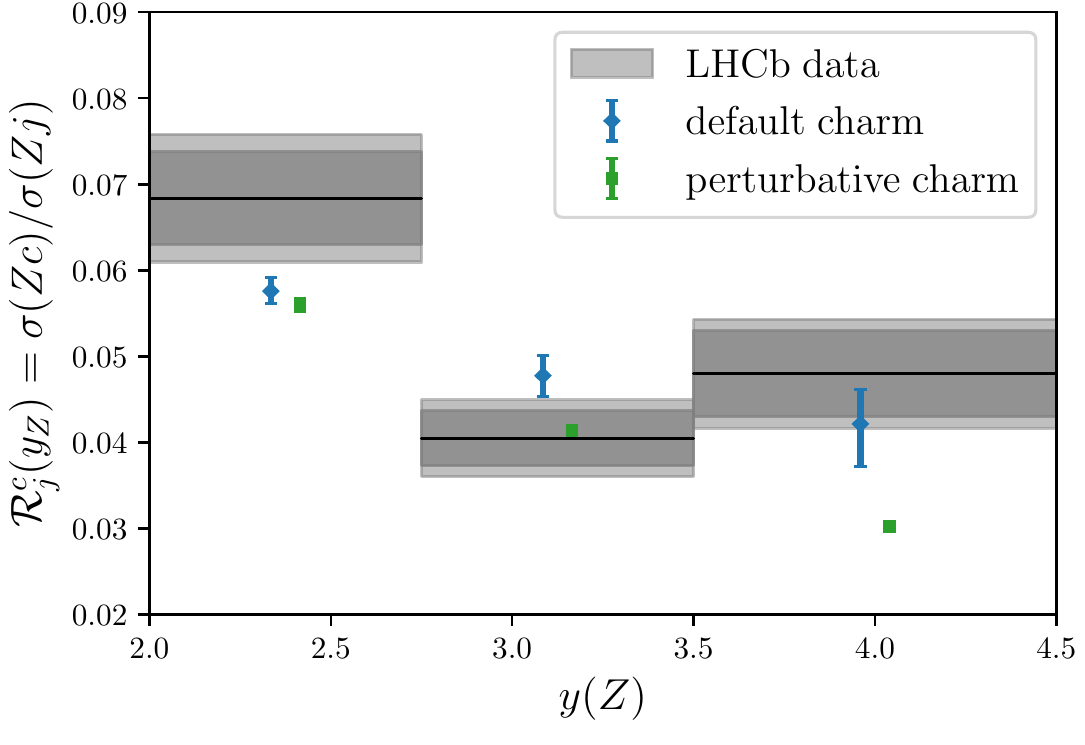
\includegraphics[width=0.6\textwidth]{lhcb_data.png}
  \end{figure}
  Assuming intrinsic charm improves prediction of recent measurement
\end{frame}

\begin{frame}{Evidence for intrinsic charm}
  \begin{figure}
    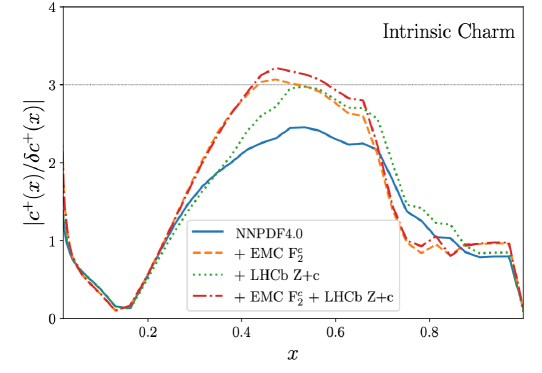
\includegraphics[width=0.45\textwidth]{ic_f2c_zc.png}
    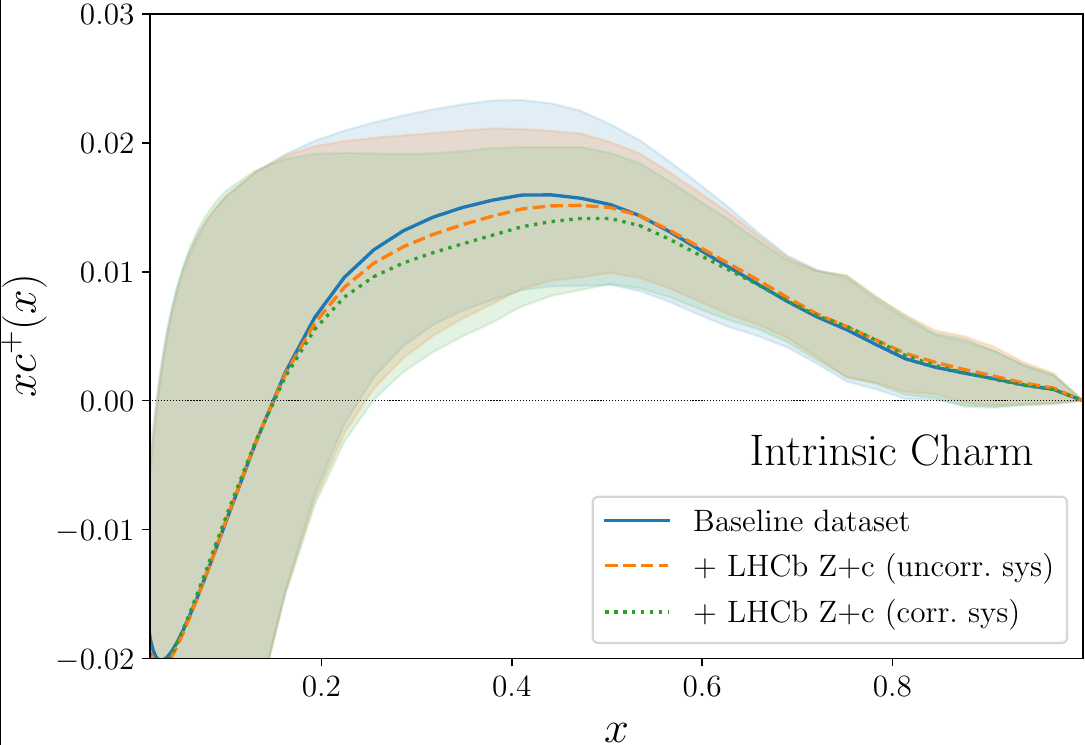
\includegraphics[width=0.45\textwidth]{lhcb_reweithed.png}
  \end{figure}
  \begin{itemize}
    \item Evidence increases upon inclusion of EMC $F_2^c$ and LHCb $Z+c$ through reweighting
  \end{itemize}
\end{frame}

\begin{frame}{Intrinsic charm at N3LO}
  \begin{itemize}
    \item Improved N3LO matching
    \item approximate N3LO PDFs $\Rightarrow$ True MHOU
    \item theory covmat MHOU included in N3LO result
    \item with MHOU: NNLO and aN3LO very colsep
  \end{itemize}
  \begin{figure}
    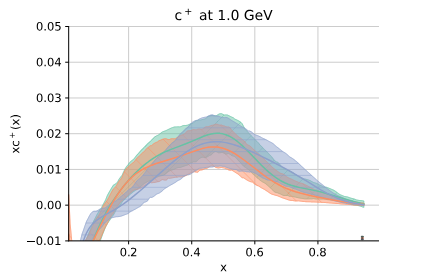
\includegraphics[width=0.45\textwidth]{n3lo_charm.png}
    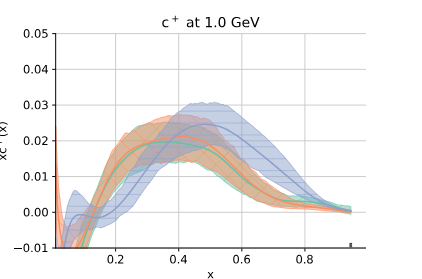
\includegraphics[width=0.45\textwidth]{n3lo_charm_mhou.png}
    \caption*{3FNS, left: no MHOU, right: with MHOU \\ green: aN3LO, orange: NNLO, blue: NLO}
  \end{figure}
\end{frame}

\begin{frame}{Intrinsic charm at N3LO}
  \begin{figure}
    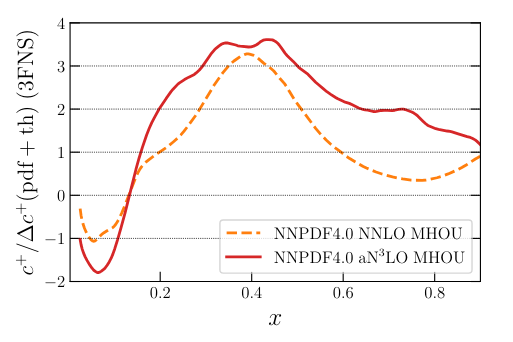
\includegraphics[width=0.6\textwidth]{n3lo_charm_pull.png}
  \end{figure}
\end{frame}

\section*{Intrinsic charm quark valence distribution of the proton}
\SectionTitleFrame[\hyperlink{https://arxiv.org/abs/2311.00743}{NNPDF, 2311.00743}]


\begin{frame}{Fitting the valence charm distribution}
  \begin{columns}
    \begin{column}{0.49\columnwidth}
      \begin{itemize}
        \item Extend fitting basis with a valence charm distribution $c^-=c-\bar{c}$
        \item Perturbative charm is generated in pair production
        \item[$\Rightarrow$] Valence charm must be intrinsic
      \end{itemize}
      \begin{figure}
        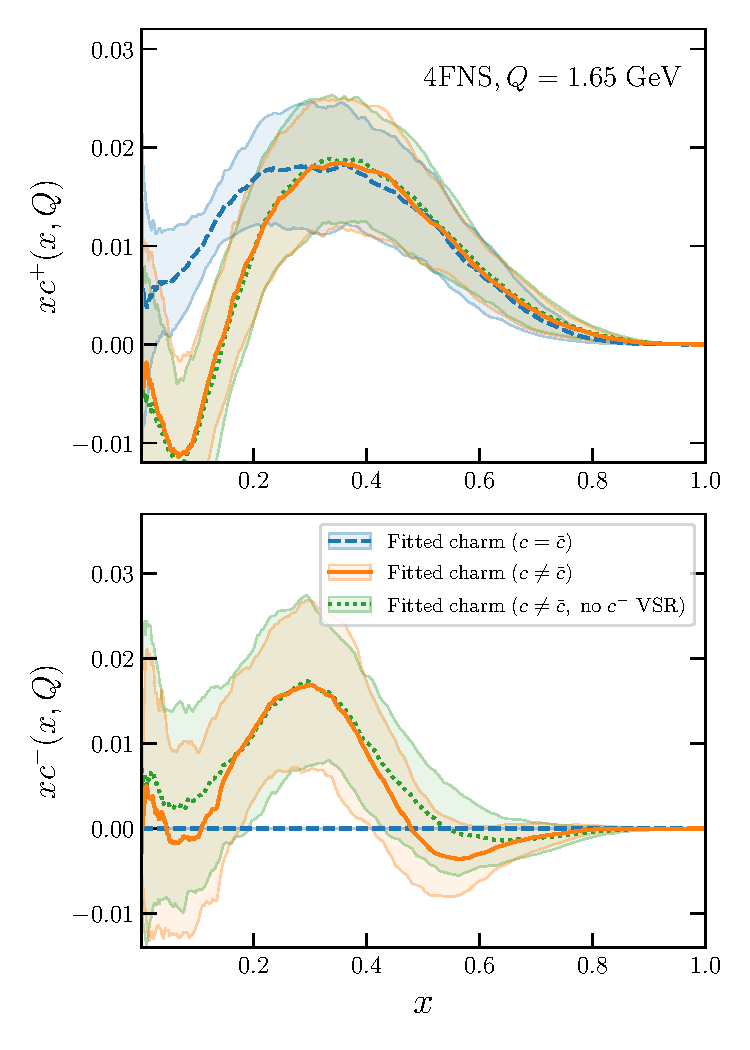
\includegraphics[width=0.6\textwidth]{CharmAsymmetry-q1p65gev-Fig1Main-noVSR.pdf}
      \end{figure}
    \end{column}
    \begin{column}{0.49\columnwidth}
      Total charm unchanged
    \end{column}
  \end{columns}
\end{frame}


\begin{frame}{Valence charm}
  \begin{itemize}
    \item Nonvanishing valance charm PDF at large-$x$
    \item Matching to $nf=3$ is perturbatively stable
  \end{itemize}
  \begin{figure}
    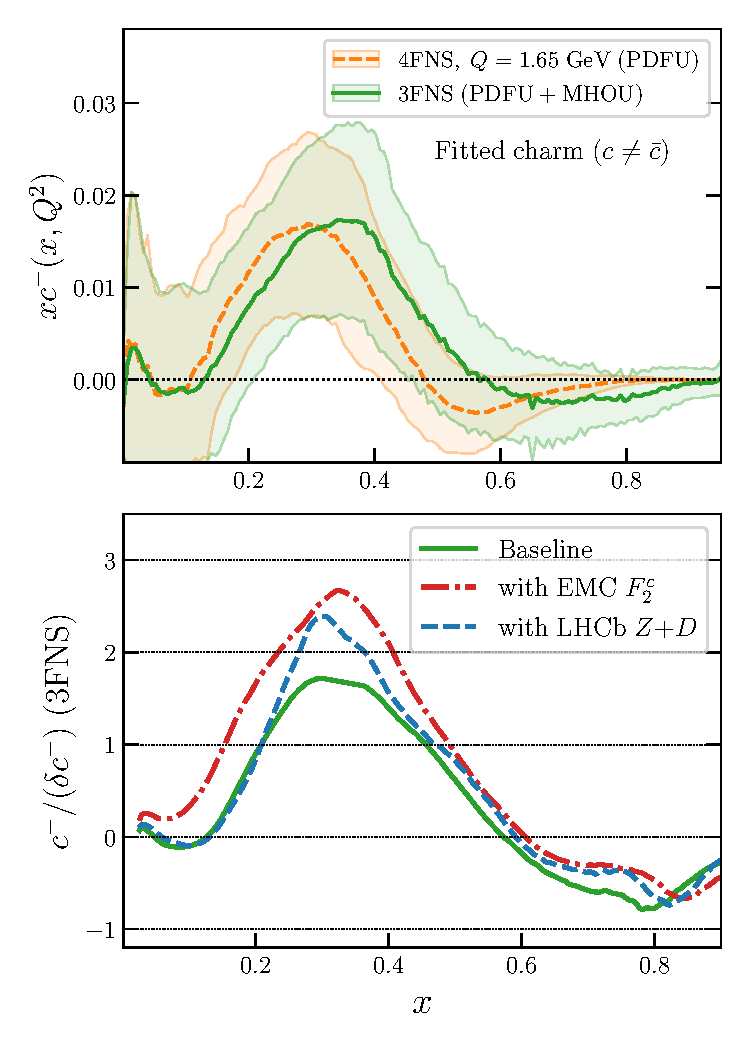
\includegraphics[width=0.6\textwidth]{CharmAsymmetryMain-3FNS-Fig2Main.pdf}
  \end{figure}
\end{frame}


\begin{frame}{Measuring the valence charm distribution at LHCb}
  Charm asymmetries in Z+c at LHCb \\
  Charm-tagged DIS at the EIC
  \begin{figure}
    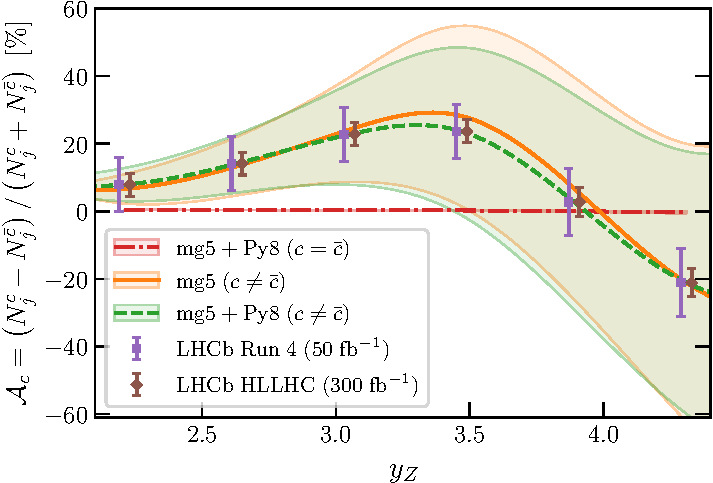
\includegraphics[width=0.45\textwidth]{lhcb-zcharm-pheno-asymm.pdf}
    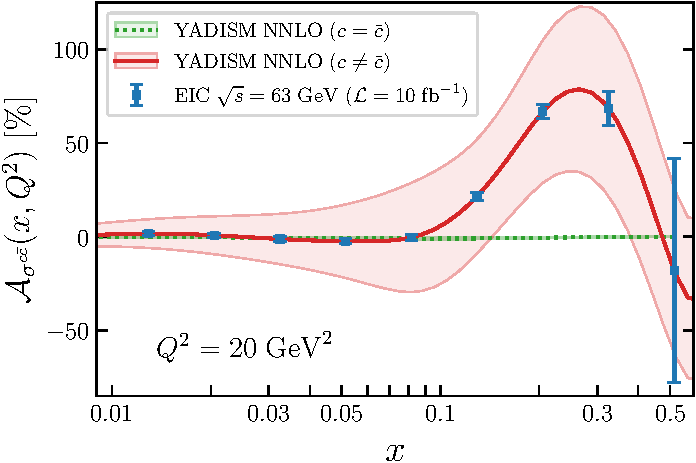
\includegraphics[width=0.45\textwidth]{ICasym-main-Fig4-EIC.pdf}
  \end{figure}
\end{frame}



\section*{PDF generalization to unseen data}
\SectionTitleFrame[\textbf{Ongoing}]

\begin{frame}{What is the impact of NNPDF4.0 uncertainties when comparing to dat not included in the fit?}
  Systematically study the impact of PDF choice in the agreement between theory and data for datasets not included in the NNPDF4.0 analysis

  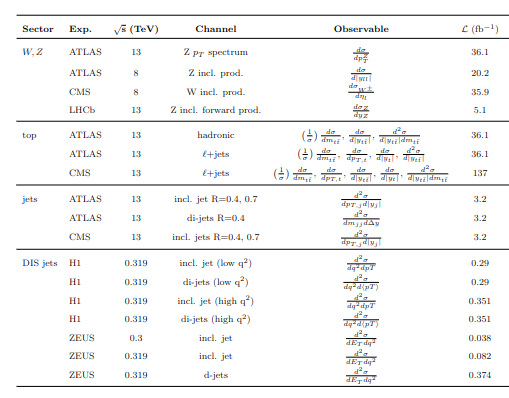
\includegraphics[width=0.6\textwidth]{pheno_paper_datastes.png}

\end{frame}

\begin{frame}{What is the impact of NNPDF4.0 uncertainties when comparing to data not included in the fit?}
  \begin{itemize}
    \item Results are full NNLO (no k-factor approximations)
    \item Baseline NNLO NNPDF4.0 (no MHOU)
  \end{itemize}

  \begin{table}[]
    \begin{tabular}{@{}lllll@{}}
    \toprule
            & CMS top $\frac{d\sigma}{dpT_t}$ &  &  &  \\ \midrule
    NNPDF4.0 & 0.768 (0.773)                        &  &  &  \\
    CT18     & 0.712 (0.729)                        &  &  &  \\
    MSHT20   & 0.699 (0.705)                        &  &  &  \\ \bottomrule
    \end{tabular}
  \end{table}


\end{frame}

\begin{frame}{A recent result from ATLAS}
  Vector boson production
  \begin{figure}
    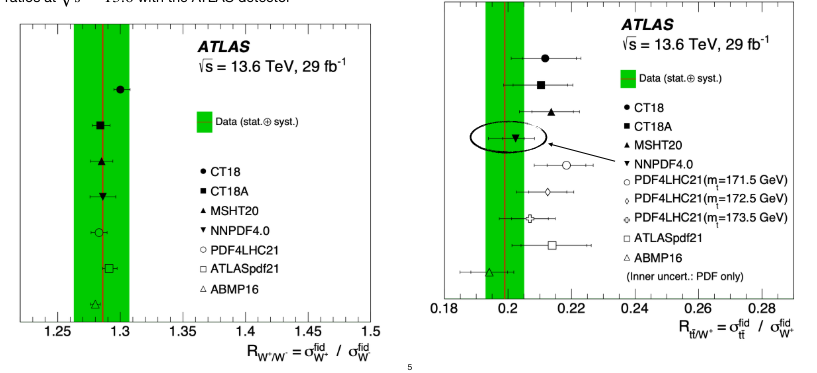
\includegraphics[width=0.6\textwidth]{atlas_vbf.png}
    \caption*{\color{gray}\footnotesize ATLAS, 2403.12902}
  \end{figure}
\end{frame}

\section{Summary}
\begin{frame}{Mesuring the valence charm distribution at LHCb}
  \begin{itemize}
    \item We fit charm to experimental data
    \item We remove the perturbative component
    \item Non-zero intrinsic charm with 3$\sigma$ significance
    \item More data: $c^+$ with 5$\sigma$ significance
    \item Need for better charmed jet definitions
  \end{itemize}

  \vspace*{5em}
  \only<2>{
    \begin{center}
      \textbf{Thank you for your attention!}
    \end{center}
  }
\end{frame}









\end{document}
